\documentclass[a5paper]{scrartcl}
\usepackage{castle_of_magic}
\usepackage{eso-pic}
\usepackage[left=0.5cm, right=0.5cm, bottom=0.4cm, top=0.5cm]{geometry}
\usepackage{multicol}
\setlength\columnsep{0.75cm}
\usepackage{enumitem}
\setmainfont{Charter}

\RedeclareSectionCommand[
  runin=false,
  beforeskip=0.0\baselineskip,
  afterskip=0.25\baselineskip
]{section}

\setkomafont{section}{\setmainfont[Scale=1.125]{Charter}\large\color{BrickRed}\bfseries}

\begin{document}
\AddToShipoutPictureBG{
\begin{tikzpicture}[remember picture, overlay]
	\node () at (current page.center) {
\includegraphics[width=\pagewidth, height=\pageheight]{Images/com_sell_sheet_background.png}};
\end{tikzpicture}
}
\begin{center}
{
\setmainfont[Scale=2.75]{Tex Gyre Chorus}
\huge
\textcolor{BrickRed}{Castle of Magic}

\normalsize

\textcolor{BrickRed}{The Card Game}
%\large
%\textcolor{BrickRed}{Castle of Magic: The Card Game}
}
\end{center}
%\vspace{-2ex}
%
\includegraphics[scale=0.125]{Images/Icons/player_count_icon.png} {\setmainfont[Scale=1.25]{Charter-Bold}\Huge \raisebox{6.55pt}{\textcolor{black}{:\ 1-6}}} \hfill 
\includegraphics[scale=0.125]{Images/Icons/player_age_icon.png} {\setmainfont[Scale=1.125]{Charter-Bold}\Huge \raisebox{6.55pt}{\textcolor{black}{:\ 8+}}}\hfill 
\includegraphics[scale=0.125]{Images/Icons/playtime_icon.png} {\setmainfont[Scale=1.125]{Charter-Bold}\Huge \raisebox{6.55pt}{\textcolor{black}{:\ 20-30}}}

\vspace{-1.75ex}
\begin{center}
\begin{tikzpicture}
\node[draw, black, ultra thick, rounded corners=3mm, text width = 0.965\textwidth, text depth=5.5ex, fill=paper!25, align=left, inner sep=0.2cm] at (0,0) {\phantom{a}A modern reimagining of a classic game of magic and intrigue. During\\\phantom{a}the game, players will assume the role of wizards who must work together\\\phantom{a}to cast a ritual spell that will determine the fate of their kingdom.};
\end{tikzpicture}
\end{center}

\raggedright
\vspace{-5ex}
\begin{multicols}{2}
\begin{tikzpicture}
\path (0,0) --++ (0, -0.5cm) node[anchor=north west, inner sep=2mm, draw, ultra thick, fill=paper!25, fill opacity=1.0, rounded corners=3mm, minimum width=1.25cm] {\tikz{
\node[inner sep=0pt] (pc) {
\includegraphics[height=1.2cm]{Images/Icons/player_count_icon_no_fill.png}};
\path (pc.south west) --++ (0, 0.08cm) node[inner sep=0pt] {\textcolor{black}{\textbf{3-6}}};
}};
\end{tikzpicture}
\hfill
\begin{tikzpicture}
\path (0,0) --++ (0, -0.5cm) node[anchor=north, inner sep=2mm, draw, ultra thick, fill=paper!25, fill opacity=1.0, rounded corners=3mm, minimum width=1.25cm] {\tikz{
\node[inner sep=0pt] (pc) {
\includegraphics[height=1.2cm]{Images/Icons/playtime_icon_no_fill.png}};
\path (pc.south) --++ (0, 0.08cm) node[inner sep=0pt] {\textcolor{black}{\textbf{30-45}}};
}};
\end{tikzpicture}
\hfill
\begin{tikzpicture}
\path (0,0) --++ (0, -0.5cm) node[anchor=north east, inner sep=2mm, draw, ultra thick, fill=paper!25, fill opacity=1.0, rounded corners=3mm, minimum width=1.25cm] {\tikz{
\node[inner sep=0pt] (pc) {
\includegraphics[height=1.2cm]{Images/Icons/player_age_icon_no_fill.png}};
\path (pc.south east) --++ (0, 0.08cm) node[inner sep=0pt] {\textcolor{black}{\textbf{12+}}};
}};
\end{tikzpicture}

\vspace{1ex}

\begin{tikzpicture}
\node[draw, black, ultra thick, rounded corners=3mm, text width = 0.56\columnwidth, fill=paper!25, align=left, inner sep = 0.2cm] at (0,0) {\vspace{-0.5ex}
\section*{\phantom{.}Components}
\begin{itemize}[nosep, leftmargin=4ex]
\vspace{-0.25ex}
\item 65 cards
\item 6 player aids
\item 12 pawns
\end{itemize}
};
\end{tikzpicture}
\hfill

\includegraphics[scale=1.0]{Images/hydra.png}
\vspace{1ex}

\begin{tikzpicture}
\node[draw, black, ultra thick, rounded corners=3mm, text width = 0.93\columnwidth, fill=paper!25, align=left, inner sep=0.2cm] at (0,0) {\vspace{-0.5ex}
\section*{\phantom{.}Story}
\vspace{-0.5ex}
\phantom{a}A Monster is imprisoned in\\\phantom{a}Castle Bondi. The shrines that\\\phantom{a}form its prison are failing. So,\\\phantom{a}wizards from three rival factions\\\phantom{a}have come together to banish the\\\phantom{a}Monster forever. The Cultists,\\\phantom{a}however, may have other plans!
};
\end{tikzpicture}
\vfill\null\columnbreak

\phantom{aj}

\vspace{0.25ex}
\begin{tikzpicture}
\node[draw, black, ultra thick, rounded corners=3mm, text width = 0.93\columnwidth, fill=paper!25, align=left, inner sep=0.2cm] at (0,0) {\vspace{-0.5ex}
\section*{\phantom{.}Gameplay}
\begin{itemize}[leftmargin=4ex, itemsep=0.2ex]
\vspace{-0.0ex}
\item Vie for control of mighty nations to secure political power for your faction.
\item Claim long-lost royal regalia\\to earn accolades for yourself. 
\item Influence mysterious and powerful arcana to shape the form of the ritual spell.
\item Banish the Monster to ensure your safety or release the Monster to rampage through the countryside.
\item Deduce which of the other wizards are allies and which are adversaries.\phantom{j}
\end{itemize}
};
\end{tikzpicture}
\end{multicols}
\begin{center}
\vspace{-3ex}
\begin{tikzpicture}
\node[draw=black, ultra thick, fill=paper!50, rounded corners=3mm] at (0,0) {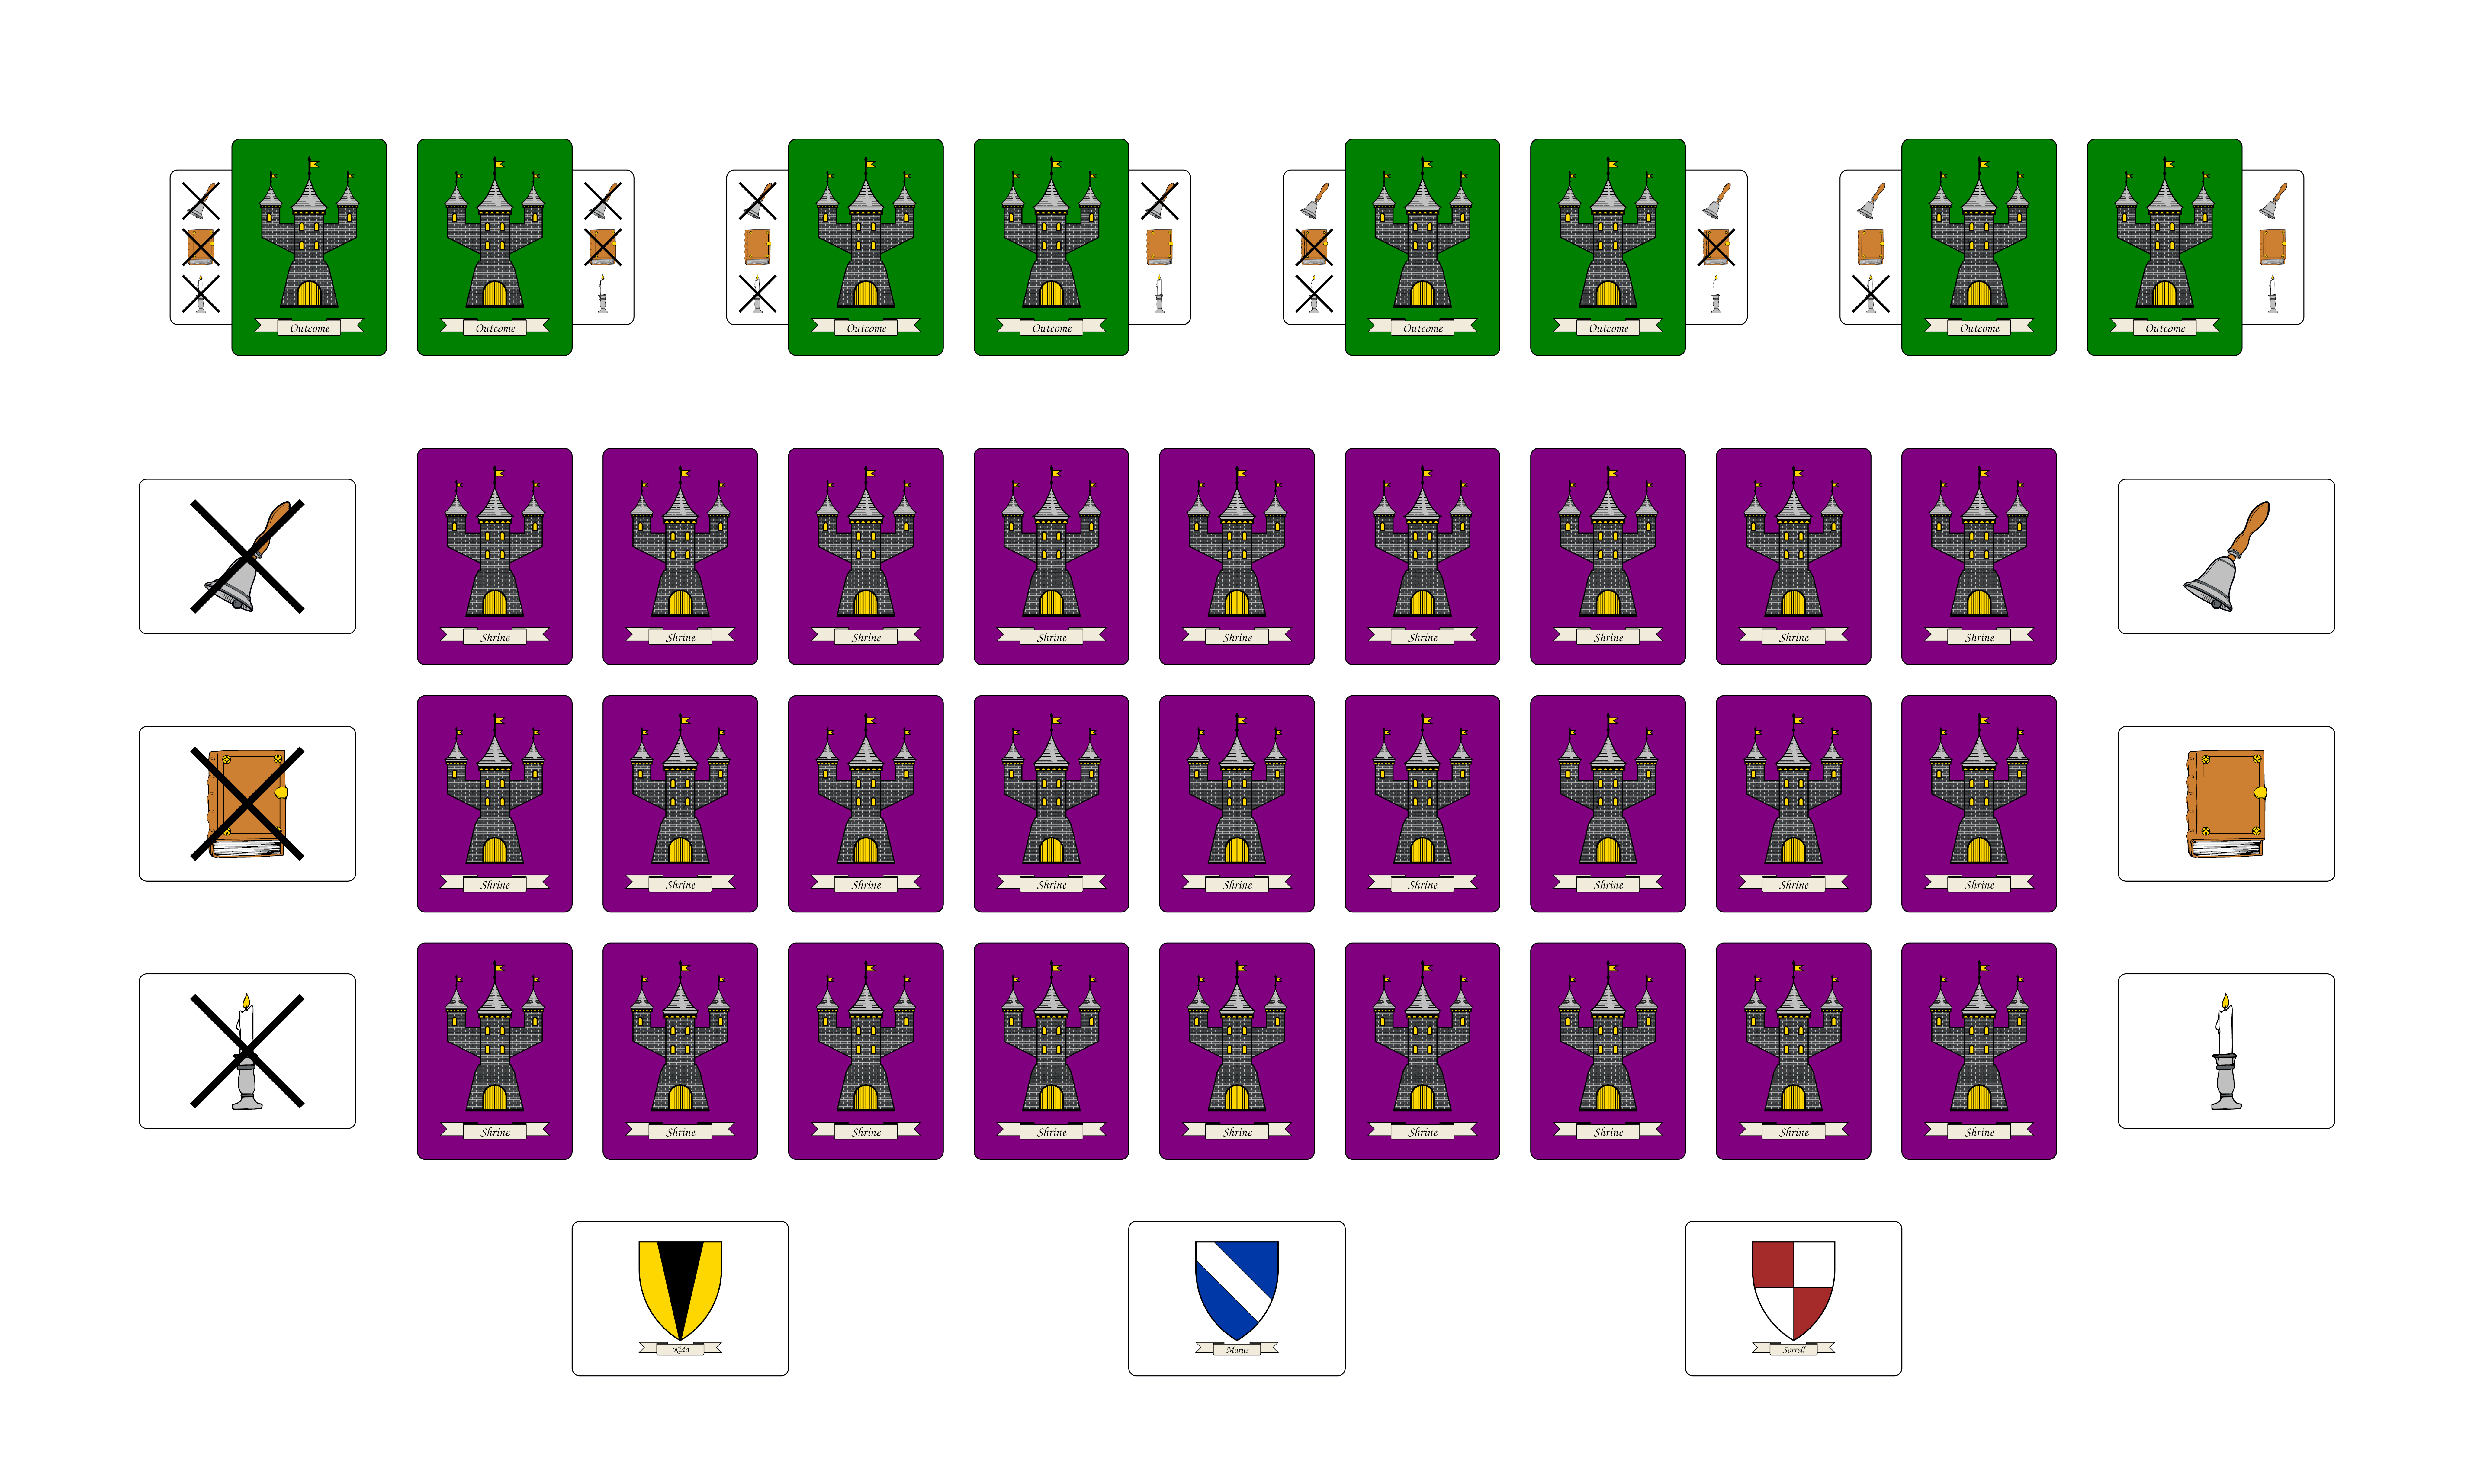
\includegraphics[width=0.5\textwidth]{Images/play_area.png}};
%\node[xscale=-1] at (-1.8in, 0) {
\includegraphics{Images/wolf_gray.png}};
%\node at (1.8in, 0) {
\includegraphics{Images/wolf_gray.png}};
\node at (-1.95in,0) {
\includegraphics[scale=1.1]{Images/dragon.png}};
\node[xscale=-1] at (1.95in, 0) {
\includegraphics[scale=1.1]{Images/dragon.png}};
\end{tikzpicture}

\medskip

\begin{tikzpicture}
\node[draw=black, ultra thick, fill=paper!50, rounded corners=3mm, text width=0.965\textwidth, text depth=0.25ex, inner sep=0.2cm] at (0,0) {\phantom{a}\textbf{Design:} Michael Purcell \hfill \textbf{Contact:} castle.of.magic.tcg@gmail.com\phantom{a}};
\end{tikzpicture}
\end{center}
%\begin{tikzpicture}
%\node[text width=127.5mm, inner sep=5mm, draw, line width=0.5mm, fill=white, fill opacity=1.0, rounded corners=1mm] (a) at (0,0) {\vspace{-2ex}\section*{Overview} A two-player card-drafting game about brass bands. During the game, players assume the roles of rival music directors who are competing to build the best band from a limited pool of local musicians.
%};
%
%\path (a.south west) --++ (0, -0.5cm) node[draw, line width=0.5mm, text width=62mm, inner sep=5mm, fill=white, fill opacity=1.0, rounded corners=1mm, anchor=north west] (b) {\vspace{-2ex}\section*{Components} 36 cards, 8 pawns, 2 score boards.};
%
%%\path (b.south) --++ (0cm, -3.25cm) node[rotate=0, transform shape] {\includegraphics[height=3.5cm]{Images/CardImages/eflat_bass_card_front.png}};
%\path (b.south west) --++ (-0.0cm, -1.3cm) node[anchor=north west, rotate=20, transform shape, inner sep=0pt] (cornet) {\includegraphics[height=3.75cm]{Images/CardImages/bass_display_front.png}};
%\path (b.south) --++ (0cm, -0.45cm) node[anchor=north, rotate=0, transform shape, inner sep=0pt] (cornet) {\includegraphics[height=3.75cm]{Images/CardImages/trombone_display_front.png}};
%\path (b.south east) --++ (0.0cm, -1.3cm) node[anchor=north east, rotate=-20, transform shape, inner sep=0pt] {\includegraphics[height=3.75cm]{Images/CardImages/cornet_display_front.png}};
%
%\path (b.south west) --++ (0cm, -5.025cm) node[anchor=north west, rotate=0, transform shape, inner sep=0pt] (s) {\includegraphics[width=72mm]{Images/score_display_front.png}};
%
%
%\path (a.south east) --++ (0, -0.5cm) node[draw, line width=0.5mm, text width=50mm, inner sep=5mm, fill=white, fill opacity=1.0, rounded corners=1mm, anchor=north east, text depth=8.7cm] (c) {\vspace{-2ex}\section*{Features} \begin{itemize}[leftmargin=*]
%\item Players draft cards to assemble eight different performances.
%\item Each performance is evaluated for its merits in four different voices.
%\item Only a player's worst voice overall determines their final score.
%\item These simple mechanics force players to make difficult choices about the tactical and strategic consequences of each card that they draft.
%%\item Tactical decisions with strategic implications.
%\end{itemize}
%};
%
%\path (s.south west) --++ (0, -0.5cm) node[anchor=north west, text width=62mm, inner sep=4.85mm, draw, line width=0.5mm, fill=white, fill opacity=1.0, rounded corners=1mm] {\textcolor{BrickRedfabric}{\textbf{\scshape{Designed By:}}} Michael Purcell\\\textcolor{BrickRedfabric}{\textbf{\scshape{Contact:}}} ttkttkt@gmail.com};
%
%\path (c.south west) --++ (0, -0.5cm) node[anchor=north west, inner sep=2mm, draw, line width=0.5mm, fill=white, fill opacity=1.0, rounded corners=1mm, minimum width=1.25cm] {\tikz{
%\node[inner sep=0pt] (pc) {\includegraphics[scale=0.125]{Images/Icons/player_count_icon_BrickRed.png}};
%\path (pc.south west) --++ (0, 0.08cm) node[inner sep=0pt] {\textcolor{BrickRedfabric}{\textbf{2}}};
%}};
%
%\path (c.south) --++ (0, -0.5cm) node[anchor=north, inner sep=2mm, draw, line width=0.5mm, fill=white, fill opacity=1.0, rounded corners=1mm, minimum width=1.25cm] {\tikz{
%\node[inner sep=0pt] (pc) {\includegraphics[scale=0.125]{Images/Icons/play_time_icon_BrickRed.png}};
%\path (pc.south) --++ (0, 0.08cm) node[inner sep=0pt] {\textcolor{BrickRedfabric}{\textbf{20-30}}};
%}};
%
%\path (c.south east) --++ (0, -0.5cm) node[anchor=north east, inner sep=2mm, draw, line width=0.5mm, fill=white, fill opacity=1.0, rounded corners=1mm, minimum width=1.25cm] {\tikz{
%\node[inner sep=0pt] (pc) {\includegraphics[scale=0.125]{Images/Icons/player_age_icon_BrickRed.png}};
%\path (pc.south east) --++ (0, 0.08cm) node[inner sep=0pt] {\textcolor{BrickRedfabric}{\textbf{12+}}};
%}};
%\end{tikzpicture}
%
\end{document}